%%%%%%%%%%%%%%%%%%%%%%%%%%%%%%%%%%%%%%%%%%%%%%%%%%%%%%%
%
% AUTHOR: 李顺
%
% DESCRIBTION: 论文第一章部分
%
%
%%%%%%%%%%%%%%%%%%%%%%%%%%%%%%%%%%%%%%%%%%%%%%%%%%%%%%%

\chapter{绪论}
\label{chap:intro}
\section{选题的背景和意义}
无人机(UAV)技术近年来发展十分迅速,其中,尤其是固定翼无人机被广泛应用于现代战争之中。但是单架无人机往往限制较多,例如
:由于机载传感器尺寸、安装位置以及精度的限制,单架无人机往往不能快速全面的侦察某一广泛区域的战略目标。

具备协同作战能力的无人机编队能更好地完成任务,与单架无人机相 比具有作战效率高、战场存活率高、
视野广阔等优势,可实现对目标的全方位立体监视,对地精确攻击,更好的完成领土保卫以及战场侦察任务。另外,无人机紧密编队可
以实现长航任务中无人机的空中加油,对接等任务, 如图\ref{fig:c01-meaning}所示。

固定翼无人机以紧密编队的形式飞行,如迁徙的鸟儿一样,可以减少整体的飞行阻力并且减少燃料消耗。整体编队产生的效果将会与精心设计的、
具有良好的气动外形的飞行器相媲美。但是,按照相关文献显示,如果固定翼编队的控制精度无法达到要求精度的10\%,那么最优的减租效果
可能会被削减30\%。\cite{Zhang2017Aerodynamics}

小型固定翼无人机具有体积小、易部署以及成本低的特点,是进行固定翼无人机编队实验的良好平台。
编队飞行作为无人机研究领域的热点与难点问题,涉及多项关键技术,例如: 队形设计、自主编队、队形保持变换、协调通信等。
 \begin{figure}[H]
  \centering
  \subfigure[无人机编队加受油]{
  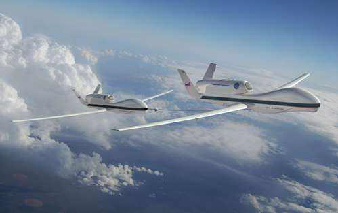
\includegraphics[width=0.45\textwidth]{figures/c1/c01-meaning-1.png} 
}
  \subfigure[无人机编队巡航]{
  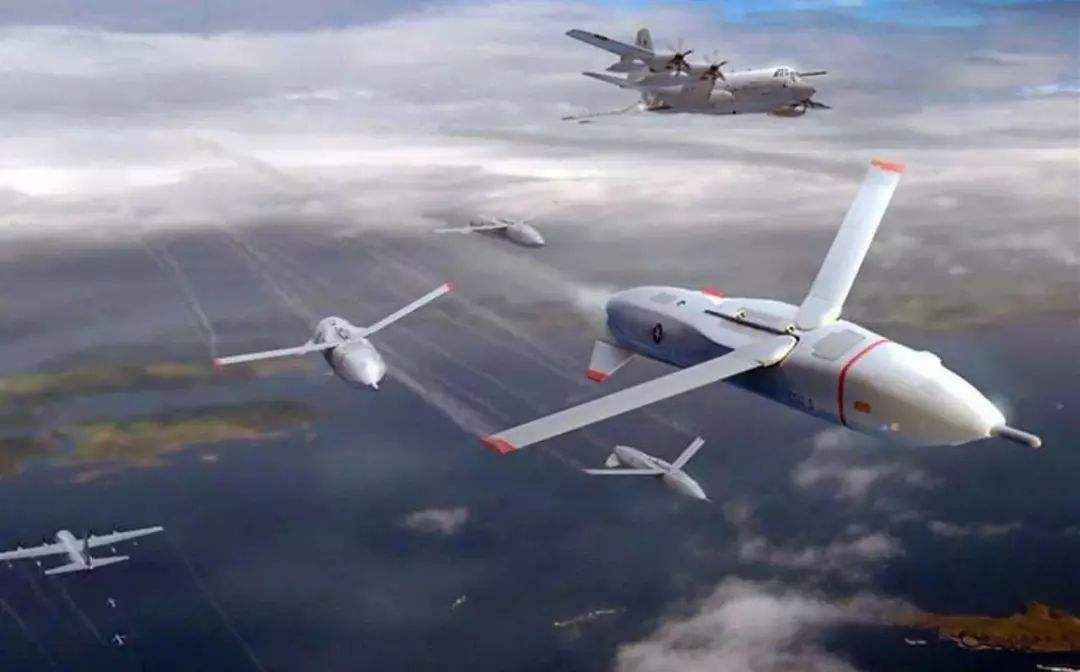
\includegraphics[width=0.45\textwidth]{figures/c1/c01-meaning-2.jpeg}
}
  \caption{无人机编队应用场景}
  \label{fig:c01-meaning}
  \end{figure}
%\upcite{Takahashi1996Structure,Xia2002Analysis,Jiang1989,Mao2000Motion,Feng1998}%这个是文献引用上标
\section{国内外研究现状及发展趋势}
%\label{sec:***} 可标注label
\subsection{无人机自动驾驶仪发展}
现如今的无人机自动驾驶仪的结构由导航模块、位置控制控制模块(外环)以及姿态控制模块(内环)组成;导航模块产生期望位置,位置控制模块由期望位置产生
期望姿态角,姿态控制模块由期望姿态角产生最终的伺服系统的控制量。现如今的低成本无人机所使用的传感器硬件精度比较低,均为消费级别,如果不考虑传感
器的精度问题而设计控制方案,很可能导致整体编队的控制精度下降。现如今已经存在的大部分编队控制算法均为考虑飞机的质点运动学以及质点动力学条件下提
出的导航方法,最终产生的飞行器的控制量为无人机航迹坐标系下的加速度期望值以及飞机的航向角的期望角速度。按照飞机的控制方式,需要将航迹坐标系下的
期望控制量转到机体系之下,但是飞机自动驾驶仪并不能接受加速度控制量,尤其是飞机机体$O_bx_b$轴方向,无人机推力、阻力以及重力沿机体方向的推力并非是代数关
系,不能直接由期望加速度得到期望推力;无人机姿态驾驶仪常使用协调转弯模型作为内环角度环的控制基础,不能直接响应所给出的偏航角速度的期望值。另外由于低成
本无人机的惯性原件的精度问题导致无人机不能使用测量的加速度信息作为反馈,两种原因导致以加速度
为最终控制量对于低成本无人机编队的方法控制精度不足。
\subsection{编队控制算法发展状况}
多无人机编队的最终目的是形成固定的亦或是随时间变化的期望几何形状。为达成此目的,目前的编队控制已经提出多种方案:
\begin{enumerate}
    \item 领从方法(leader-follower method) 此种方法本质而言是基于距离的编队方法(distance-based),因其原理简单,而得到广泛应用。
        领从方法的大致思路为:领航无人机按照预先设定的轨迹飞行,跟随无人机以期望编队位置的距离误差,与领航无人机速度误差作为误差
        输入,最终使得误差消除,达到编队目的。2008年,王莉等对多无人车系统进行编队算法设计。2012年,宾西法尼亚大学的Turpin等
        提出了改进leader-follower 编队算法,每架无人机从与之通信的邻居无人机中间接获取领航无人机的状态信息。团队小组Saska等
        基于机载感知设备实现非GPS定位的密集飞行任务。
    \item 基于行为方法
        此种方法将无人机的完整任务划分为几种多种行为,例如:跟随、队形保持、队形变换以及避障等。对于不同行为的加权作为最终无人机的
        “控制行为”。1998年,Arkin等人提出了一种基于行为的编队控制算法,解决多智能体编队控制问题。2009年,R.K.Sharma等人将基于行为
        法改进,用来解决编队控制中的避障问题。近年来,有学者对生物行为进行分析学习,并通过类似行为分析的方法引入编队控制中
        2003年,美国 Jadbabaie 等人提出了最近邻近协调的思想,为了对基于行为法进行深入的研究。Lin等在2009年设计出一种基于反馈线
        性化方法设计的分布式控制器。河南理工大学宋运忠等在2012 年,利用线性手段解非线性的物理模型方程,解决了多智能体系统队形控
        制问题,改进了智能体行为的方法。近年来仿生学的发展为这一技术提供契机。2015年,段海滨等建立了鸽群行为机制模型,提出了鸽群
        行为编队控制算法。为了提高人机群集编队的鲁棒性,Shin等在同一年提出了分布式编队控制策略,主要处理相邻无人机状态信息。
    \item 虚拟结构法
        算法思路是将编队看作虚拟刚体,假设虚拟刚体中有一个虚拟主机或几何中心,刚体中的所有无人机都围绕主机或虚拟几何中心移动[20]
        。算法最初是用于集中式算法设计中,随着科技发展,也有研究者用分布式算法对虚拟结构法进行分布式设计。
        任伟等结合一致性算法与虚拟结构法,对带干扰的便对运动问题进行反馈控制求解[21];在另一篇论文中,任伟结合一致性算法与虚拟结
        构法,对集中式的虚拟结构法进行分布式求解,提出了分布式算法解决编队问题。
\end{enumerate}
\section{本文的内容安排}
本文中的编队控制器设计主要基于领从方法,从无人机编队的距离、速度大小以及速度方向误差出发,设计符合现有无人机内环姿态驾驶仪输入的
编队控制器。
本文之后的部分将如下组织:第二章首先介绍编队控制设计的假设以及所用到的坐标系,最终建立建立无人机编队的动力学模型;第三章首先
完成对于编队误差的定义,将所定义的编队误差作为输入、无人机内环姿态驾驶仪期望姿态作为输出,设计编队控制器数学形式;第四章介绍
无人机编队整体控制逻辑、动力学仿真环境以及硬件选型 ;第五章控制器仿真以及实际飞行实验结果分析;第六章为结论。
